\documentclass[11pt,a4paper]{article}
\usepackage[utf8]{inputenc}
\usepackage[T1]{fontenc}
\usepackage[norsk]{babel}
\usepackage{tgtermes}
\usepackage{tgheros}
\renewcommand{\ttdefault}{txtt}
\usepackage{amsmath,amssymb}
\usepackage[a4paper,left=2.45cm,right=2.6cm,top=2.3cm,bottom=2.2cm,headsep=0.9cm]{geometry}
\usepackage{fancyhdr}
\usepackage{lastpage}
\usepackage{xcolor}
\usepackage{tikz}
\usepackage{pgfplots}
\pgfplotsset{compat=1.18}
\usepackage{booktabs}
\usepackage{array}
\usepackage{enumitem}
\usepackage{listings}
\usepackage{needspace}
\usepackage{multirow}
\usetikzlibrary{positioning,arrows.meta,calc}
\definecolor{insgrey}{gray}{0.42}
\definecolor{radiogrey}{gray}{0.70}
\setlength{\parindent}{0pt}
\setlength{\parskip}{0.45em}
\setlist[itemize]{itemsep=0pt,topsep=2pt,label=\textbullet,font=\sffamily}
\lstset{basicstyle=\ttfamily\small,columns=fullflexible,keepspaces=true,
  showstringspaces=false,upquote=true,aboveskip=0.6em,belowskip=0.6em,
  literate={æ}{{\ae}}1 {ø}{{\o}}1 {å}{{\aa}}1 {Æ}{{\AE}}1 {Ø}{{\O}}1 {Å}{{\AA}}1}
\pagestyle{fancy}
\fancyhf{}
\renewcommand{\headrulewidth}{0pt}
\fancyhead[R]{\fontsize{7.5}{9}\selectfont\sffamily\color{insgrey}TDT4172 - Introduksjon til maskinlæring - Øvingssett 2}
\fancyfoot[R]{\fontsize{7}{9}\selectfont\sffamily\color{insgrey}\thepage/\pageref{LastPage}}
\newcommand{\delstart}[1]{\clearpage
  \noindent\hspace*{-1.55em}\makebox[1.55em][l]{\sffamily\bfseries\fontsize{12}{14}\selectfont\raisebox{0.35em}{#1}}%
  {\sffamily\bfseries\fontsize{18}{22}\selectfont Part #1}\par\vspace{1.0em}}
\newcommand{\sporsmal}[1]{\par\Needspace{9\baselineskip}\vspace{1.9em}%
  \noindent{\bfseries Spørsmål #1}\par\vspace{-0.45em}%
  \noindent{\bfseries -{}-{}-{}-{}-{}-{}-{}-{}-{}-{}-{}-{}-{}-{}-{}-{}-}\par\vspace{-0.15em}}
\newcommand{\velg}[1]{\par\Needspace{6\baselineskip}\noindent{\bfseries #1}\par\vspace{0.3em}}
\newcommand{\radio}[1]{\tikz[baseline=-0.62ex]{\draw[radiogrey,line width=0.45pt,fill=gray!5] (0,0) circle (0.56em);
  \node[inner sep=0pt,font=\sffamily\fontsize{5.5}{6}\selectfont,text=insgrey] at (0,0) {#1};}}
\newenvironment{alternativer}{\begin{list}{}{\setlength{\leftmargin}{2.35em}\setlength{\labelwidth}{1.4em}%
  \setlength{\labelsep}{0.6em}\setlength{\itemsep}{0.85em}\setlength{\topsep}{0.45em}\setlength{\parsep}{0pt}}%
  \sffamily\fontsize{10}{12.6}\selectfont}{\end{list}}
\newcommand{\alt}[2]{\item[\radio{#1}]#2}
\newcommand{\makspoeng}{\par\vspace{2.2em}\hfill{\sffamily\fontsize{8.5}{10}\selectfont Maks poeng: 10}\hspace*{0.5em}\par}
\begin{document}

\noindent\hspace*{-1.55em}\makebox[1.55em][l]{\raisebox{0.3em}{\sffamily\bfseries\fontsize{11}{12}\selectfont i}}%
{\sffamily\bfseries\fontsize{18}{22}\selectfont Frontpage}\par\vspace{1.1em}

{\bfseries Eksamensoppgave i TDT4172 - Introduksjon til maskinlæring}\\
{\bfseries Øvingssett:} 2 av 10 (uoffisielt øvingssett)\\
{\bfseries Tid:} 4 timer

\vspace{0.6em}
{\bfseries Faglig kontakt:} --- (øvingssett, ikke en offisiell eksamen)\\
{\bfseries Møter i eksamenslokalet:} Nei

\vspace{0.6em}
{\bfseries Hjelpemiddelkode/Tillatte hjelpemidler:} D / Ingen trykte eller håndskrevne hjelpemidler tillatt.
Bestemt, enkel kalkulator tillatt.

\vspace{0.6em}
{\bfseries\underline{ANNEN INFORMASJON:}}

\vspace{0.4em}
{\bfseries Les oppgavene nøye og gjør dine egne antagelser.} Presiser i besvarelsen hvilke forutsetninger du
har lagt til grunn i tolkning/avgrensing av oppgaven.

Dette øvingssettet er laget for egentrening, med samme format og vanskelighetsgrad som de
siste ordinære eksamenene i emnet. Løsningsforslaget står på siste side.

\vspace{1.6em}
{\bfseries\underline{FAGSPESIFIKK INFORMASJON}}

\vspace{0.4em}
{\bfseries Ingen papirhåndtegninger:}\\
Denne eksamenen tillater ikke bruk av håndtegninger.

\vspace{1.4em}
{\bfseries Vekting av oppgavene}:\\
Denne eksamenen inneholder flervalgsoppgaver organisert i ti grupper på fire spørsmål hver. Hver
gruppe vurderes separat etter følgende regler:

\vspace{0.6em}
For hver av de fire spørsmålene i gruppen får du følgende poeng
\begin{itemize}[leftmargin=2.2em,label=\textperiodcentered,itemsep=0pt]
\item {\bfseries Riktig svar:} +2,5 poeng
\item {\bfseries Feil svar (et alternativ er valgt, men ikke korrekt):} $-$0,83 poeng
\item {\bfseries Ikke besvart:} 0 poeng
\end{itemize}
{\bfseries Merk} at dersom du først har valgt et svaralternativ, kan du {\bfseries ikke velge det bort} igjen. Da må du
svare på det spørsmålet. Med andre ord mister du muligheten til å la et spørsmål stå blankt så fort
du har trykket på et alternativ.

\vspace{0.6em}
Poengsummen for hver gruppe er {\bfseries summen} av poengene for de fire enkeltspørsmålene.\\
For {\bfseries alle spørsmålene} gjelder en {\bfseries null-grense}: dersom summen for denne gruppen blir negativ,
settes verdien til {\bfseries 0}. Den totale poengsummen på eksamen er summen av poengene fra alle
gruppene.

\delstart{1}
\sporsmal{1}
Featuren \emph{Alder} har gjennomsnitt 40 og standardavvik 8 i treningssettet, og gjennomsnitt 45 og
standardavvik 10 i testsettet. Du kjører
\begin{lstlisting}[language=Python]
scaler = StandardScaler().fit(X_train)
X_test_s = scaler.transform(X_test)
\end{lstlisting}

Hvilken verdi får et testpunkt med \emph{Alder} $= 58$?
\velg{Velg ett alternativ:}
\begin{alternativer}
\alt{A}{$0.45$}
\alt{B}{$1.30$}
\alt{C}{$0.28$}
\alt{D}{$2.25$}
\end{alternativer}
\sporsmal{2}
En logistisk regresjonsmodell har bias $b = 0.2$ og trenes med full-batch gradient descent med
læringsrate $\eta = 0.3$. Gradienten av gjennomsnittlig cross-entropy-tap med hensyn på $b$ er
\[ \frac{\partial L}{\partial b} = \frac{1}{N}\sum_{i=1}^{N}\big(\hat y^{(i)} - y^{(i)}\big). \]
For de tre treningspunktene er $\hat y = (0.8,\ 0.3,\ 0.6)$ og $y = (1,\ 0,\ 0)$.

Hva blir $b$ etter ett gradient descent-steg?
\velg{Velg ett alternativ:}
\begin{alternativer}
\alt{A}{$-0.01$}
\alt{B}{$-0.03$}
\alt{C}{$0.09$}
\alt{D}{$0.13$}
\end{alternativer}
\sporsmal{3}
I notatene utledes cross-entropy loss fra likelihooden
$L(\mathbf{w}, b \mid \mathbf{x}, y) = \sigma(\mathbf{w}\mathbf{x}+b)^{y}\,\big(1-\sigma(\mathbf{w}\mathbf{x}+b)\big)^{1-y}$:
først tas logaritmen, og deretter settes et minustegn foran.

Hvilket utsagn begrunner disse to stegene riktig?
\velg{Velg ett alternativ:}
\begin{alternativer}
\alt{A}{Logaritmen flytter optimum til et punkt som er enklere å finne; minustegnet gjør tapet til en sannsynlighet}
\alt{B}{Logaritmen er monoton og flytter ikke optimum; minustegnet gjør en maksimering om til en minimering}
\alt{C}{Logaritmen gjør likelihooden konveks; minustegnet trengs fordi logaritmen av en sannsynlighet er positiv}
\alt{D}{Logaritmen trengs for at gradienten skal eksistere; minustegnet får gradienten til å peke mot optimum}
\end{alternativer}
\sporsmal{4}
Et nevralt nettverk for tre klasser har softmax i output-laget. For ett datapunkt er verdiene inn til
softmax (logits) $\mathbf{z} = (2.0,\ 1.0,\ 0.0)$, og riktig klasse er klasse 2 (den midterste), dvs.\
$\mathbf{y} = (0,\,1,\,0)$.

Hva blir kategorisk cross-entropy $L = -\sum_i y_i \ln \hat y_i$ for dette datapunktet?
\velg{Velg ett alternativ:}
\begin{alternativer}
\alt{A}{$0.41$}
\alt{B}{$2.41$}
\alt{C}{$1.41$}
\alt{D}{$0.61$}
\end{alternativer}
\makspoeng

\delstart{2}
\sporsmal{1}
Et datasett med 10\,000 korttransaksjoner inneholder 150 svindeltilfeller (positiv klasse).
En modell predikerer «ikke svindel» for alle transaksjonene.

Hvilket utsagn om modellen er riktig?
\velg{Velg ett alternativ:}
\begin{alternativer}
\alt{A}{Accuracy er 98.5\,\%, og F1-scoren er nær 1, siden modellen aldri gir en falsk alarm}
\alt{B}{Accuracy er 98.5\,\%, men spesifisiteten er 0, siden modellen aldri predikerer positiv klasse}
\alt{C}{Accuracy er 98.5\,\%, og recall er også 98.5\,\%, siden nesten alle tilfeller klassifiseres riktig}
\alt{D}{Accuracy er 98.5\,\%, men recall er 0, siden modellen ikke finner noen av svindeltilfellene}
\end{alternativer}
\sporsmal{2}
Et e-postsystem skal flytte phishing-e-poster (positiv klasse) til en karantene som brukerne aldri ser.
En legitim e-post som havner i karantenen, er dermed tapt for mottakeren, og dette er svært kostbart.
En phishing-e-post som slipper gjennom, blir som regel stoppet av andre sikkerhetstiltak.

Hvilken metrikk bør modellen først og fremst skåre høyt på?
\velg{Velg ett alternativ:}
\begin{alternativer}
\alt{A}{Precision, fordi falske negative er den dyreste feiltypen her}
\alt{B}{Recall, fordi falske negative er den dyreste feiltypen her}
\alt{C}{Recall, fordi falske positive er den dyreste feiltypen her}
\alt{D}{Precision, fordi falske positive er den dyreste feiltypen her}
\end{alternativer}
\sporsmal{3}
En binær klassifikator gir følgende prediksjoner på ti testpunkter (1 = positiv klasse):
\begin{center}
\begin{tabular}{lcccccccccc}
\toprule
Punkt & 1 & 2 & 3 & 4 & 5 & 6 & 7 & 8 & 9 & 10\\
\midrule
Label $y$ & 1 & 0 & 1 & 1 & 0 & 0 & 1 & 0 & 1 & 0\\
Prediksjon $\hat y$ & 1 & 0 & 0 & 1 & 1 & 0 & 1 & 0 & 0 & 0\\
\bottomrule
\end{tabular}
\end{center}
Hva blir confusion matrix-verdiene?
\velg{Velg ett alternativ:}
\begin{alternativer}
\alt{A}{TP $= 4$, FP $= 1$, FN $= 2$, TN $= 3$}
\alt{B}{TP $= 3$, FP $= 1$, FN $= 2$, TN $= 4$}
\alt{C}{TP $= 4$, FP $= 2$, FN $= 1$, TN $= 3$}
\alt{D}{TP $= 3$, FP $= 2$, FN $= 1$, TN $= 4$}
\end{alternativer}
\sporsmal{4}
Du har delt dataene i trening, validering og test. Etter treningen prøver du 20 ulike
klassifiseringsterskler, velger terskelen som gir høyest F1-score på \textbf{testsettet}, og rapporterer
denne F1-scoren som modellens ytelse.

Hva er problemet med denne fremgangsmåten?
\velg{Velg ett alternativ:}
\begin{alternativer}
\alt{A}{Ingen problemer, siden terskelen ikke endrer modellens parametre og derfor kan velges på testsettet}
\alt{B}{Terskelen burde vært valgt på treningssettet, siden modellen er tilpasset de samme dataene}
\alt{C}{F1 er feil metrikk; med accuracy ville fremgangsmåten gitt et forventningsrett ytelsesestimat}
\alt{D}{Den rapporterte F1-scoren blir for optimistisk, siden testsettet er brukt til å velge terskelen}
\end{alternativer}
\makspoeng

\delstart{3}
\sporsmal{1}
En node i et klassifikasjonstre har punkter fra fire klasser med andelene $(0.5,\ 0.25,\ 0.125,\ 0.125)$.

Hva er entropien $I = -\sum_i p_i \log_2 p_i$ i noden?
\velg{Velg ett alternativ:}
\begin{alternativer}
\alt{A}{$1.21$}
\alt{B}{$1.00$}
\alt{C}{$1.75$}
\alt{D}{$0.66$}
\end{alternativer}
\sporsmal{2}
Du bruker Naive Bayes på Titanic-dataene med features $x_1 = $ \emph{Pclass} og $x_2 = $ \emph{Sex}
for å predikere klassen $C_k$ (\emph{Survived}).

Hvilken antakelse gjør modellen?
\velg{Velg ett alternativ:}
\begin{alternativer}
\alt{A}{$p(x_1, x_2 \mid C_k) = p(x_1 \mid C_k)\,p(x_2 \mid C_k)$ for hver klasse $C_k$}
\alt{B}{$p(x_1, x_2 \mid C_k) = p(x_1 \mid C_k) + p(x_2 \mid C_k)$ for hver klasse $C_k$}
\alt{C}{$p(C_k \mid x_1, x_2) = p(C_k \mid x_1)\,p(C_k \mid x_2)$ for hver klasse $C_k$}
\alt{D}{$p(x_1, x_2 \mid C_k) = p(x_1 \mid C_k)\,p(x_2)$ for hver klasse $C_k$}
\end{alternativer}
\sporsmal{3}
Når et beslutningstre velger splitt i en node, kan det enten maksimere informasjonsgevinsten
$\Delta I = I_{\text{før}} - E[I_{\text{etter}}]$ eller minimere den vektede entropien etter splitten,
$E[I_{\text{etter}}]$.

Hvilket utsagn om disse to kriteriene er riktig?
\velg{Velg ett alternativ:}
\begin{alternativer}
\alt{A}{De gir alltid identisk valg, siden $I_{\text{før}}$ er felles for alle kandidatene i noden}
\alt{B}{Bare $\Delta I$ vekter barnenodene etter antall punkter, så kriteriene kan skille seg i ubalanserte splitter}
\alt{C}{De faller sammen bare når foreldrenoden har like mange punkter fra hver klasse, slik at $I_{\text{før}} = 1$}
\alt{D}{De gir identisk valg med entropi, men med Gini som urenhetsmål kan de to kriteriene velge ulike splitter}
\end{alternativer}
\sporsmal{4}
Et klassifikasjonstre har binære splitter (hver beslutningsnode har to barn) og \texttt{max\_depth=4}, der
rotnoden har dybde 0.

Hvor mange løvnoder, og dermed ulike regioner i datarommet, kan treet maksimalt ha?
\velg{Velg ett alternativ:}
\begin{alternativer}
\alt{A}{$4$}
\alt{B}{$8$}
\alt{C}{$15$}
\alt{D}{$16$}
\end{alternativer}
\makspoeng

\delstart{4}
\sporsmal{1}
Du tilpasser modellen $f(x) = \beta_0 + \beta_1 x + \beta_2 x^2$ til data med én feature $x$.

Hvilket utsagn er riktig?
\velg{Velg ett alternativ:}
\begin{alternativer}
\alt{A}{Modellen er lineær i parametrene bare dersom $x$ først standardiseres til gjennomsnitt 0}
\alt{B}{Modellen er ikke-lineær i parametrene, så MSE-tapet er ikke lenger konvekst i $\beta_0$, $\beta_1$ og $\beta_2$}
\alt{C}{Modellen er lineær i parametrene og kan trenes som lineær regresjon med $x$ og $x^2$ som features}
\alt{D}{Modellen må trenes som et nevralt nettverk, siden lineær regresjon bare kan tilpasse rette linjer}
\end{alternativer}
\sporsmal{2}
Du skal tilpasse en polynomisk regresjonsmodell og vil velge graden $M \in \{1, 2, \ldots, 15\}$.
Dataene er delt i trening, validering og test.

Hvilken fremgangsmåte er riktig?
\velg{Velg ett alternativ:}
\begin{alternativer}
\alt{A}{$M$ er en modellparameter; la gradient descent lære $M$ sammen med koeffisientene $\beta_i$}
\alt{B}{$M$ er en hyperparameter; tren én modell per grad og velg den som gir lavest tap på testdataene}
\alt{C}{$M$ er en hyperparameter; tren én modell per grad og velg den med lavest tap på treningsdataene}
\alt{D}{$M$ er en hyperparameter; tren én modell per grad og velg den med lavest tap på valideringsdata}
\end{alternativer}
\sporsmal{3}
Figuren viser et \textbf{regresjonstre} med dybde 2. Hver node viser splittregelen (indre noder), antall
treningspunkter $n$ og gjennomsnittet av target for treningspunktene i noden. Venstre gren følges når
splittregelen er oppfylt.
\begin{center}
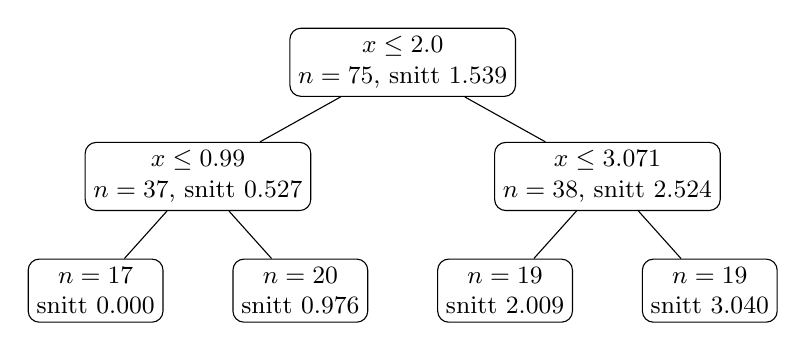
\begin{tikzpicture}[level distance=1.45cm,
  level 1/.style={sibling distance=5.2cm}, level 2/.style={sibling distance=2.6cm},
  every node/.style={draw, rounded corners, align=center, font=\small, inner sep=3pt}]
\node {$x \le 2.0$\\ $n=75$, snitt $1.539$}
  child {node {$x \le 0.99$\\ $n=37$, snitt $0.527$}
    child {node {$n=17$\\ snitt $0.000$}}
    child {node {$n=20$\\ snitt $0.976$}}}
  child {node {$x \le 3.071$\\ $n=38$, snitt $2.524$}
    child {node {$n=19$\\ snitt $2.009$}}
    child {node {$n=19$\\ snitt $3.040$}}};
\end{tikzpicture}
\end{center}
Hva predikerer treet for et nytt punkt med $x = 3.5$?
\velg{Velg ett alternativ:}
\begin{alternativer}
\alt{A}{$3.040$}
\alt{B}{$2.009$}
\alt{C}{$1.539$}
\alt{D}{$2.524$}
\end{alternativer}
\sporsmal{4}
En konstant modell $f(x) = c$ tilpasses ved å minimere MSE på target-verdiene $\{1,\ 2,\ 3,\ 4,\ 100\}$.

Hvor stor andel av den totale kvadrerte feilen $\sum_i (y_i - c)^2$ ved den optimale $c$ kommer fra
punktet $y = 100$?
\velg{Velg ett alternativ:}
\begin{alternativer}
\alt{A}{$0.50$}
\alt{B}{$0.80$}
\alt{C}{$1.00$}
\alt{D}{$0.20$}
\end{alternativer}
\makspoeng

\delstart{5}
\sporsmal{1}
Fra et treningssett med $n = 1000$ ulike punkter trekkes et bootstrap-utvalg av størrelse 1000. Et bestemt
punkt kommer med minst én gang med sannsynlighet $1-(1-1/n)^n \approx 0.632$, og over alle trekninger
forekommer hvert punkt i snitt én gang i utvalget.

Hvor mange ganger forekommer punktet i snitt, \textbf{gitt at} det er med i utvalget?
\velg{Velg ett alternativ:}
\begin{alternativer}
\alt{A}{$1.58$}
\alt{B}{$0.37$}
\alt{C}{$1.00$}
\alt{D}{$0.63$}
\end{alternativer}
\sporsmal{2}
Sammenhengen mellom features og target er tilnærmet lineær for noen features, men har skarpe
terskeleffekter for andre. Du sammenligner en lineær regresjonsmodell, et regresjonstre og et parallelt
ensemble som tar gjennomsnittet av de to modellenes prediksjoner.

Hvorfor kan ensemblet gjøre det bedre enn begge enkeltmodellene?
\velg{Velg ett alternativ:}
\begin{alternativer}
\alt{A}{Gjennomsnittet av en lineær modell og et tre er selv lineært, men har lavere varians enn hver av dem}
\alt{B}{Modellene bygger på ulike antakelser (lineær form og akseparallelle splitter) og gjør derfor ulike feil}
\alt{C}{Treet retter opp feilene til den lineære modellen, siden det trenes på residualene fra den}
\alt{D}{Gjennomsnittet halverer variansen, siden prediksjonene fra ulike modelltyper er uavhengige}
\end{alternativer}
\sporsmal{3}
Tre klassifikatorer har hver 70\,\% accuracy, og feilene deres er uavhengige av hverandre. De kombineres
med flertallsavstemning.

Hva er sannsynligheten for at ensemblet klassifiserer et tilfeldig punkt riktig?
\velg{Velg ett alternativ:}
\begin{alternativer}
\alt{A}{$0.78$}
\alt{B}{$0.34$}
\alt{C}{$0.44$}
\alt{D}{$0.70$}
\end{alternativer}
\sporsmal{4}
Gradient boosting har fått navnet sitt fra gradient descent.

Hvilket utsagn beskriver sammenhengen riktig?
\velg{Velg ett alternativ:}
\begin{alternativer}
\alt{A}{Læringsraten og trædybden justeres langs gradienten av valideringstapet etter hver runde med et nytt tre}
\alt{B}{Hvert nye tre tilpasses den negative gradienten av tapet mht.\ prediksjonene, for kvadratisk tap residualene}
\alt{C}{Vektene til feilpredikerte punkter økes langs gradienten av tapet i hver runde, så neste tre fokuserer på dem}
\alt{D}{Splittverdiene i ett stort tre justeres med gradient descent i hver runde, slik at tapet på treningsdataene synker}
\end{alternativer}
\makspoeng

\delstart{6}
\sporsmal{1}
Et perceptron med to binære input $x_1, x_2 \in \{0, 1\}$ har vekter $w_1 = w_2 = -1$, bias $b = 1.5$ og
aktiveringsfunksjonen $H(z) = 1$ hvis $z \geq 0$, ellers $0$, der $z = w_1x_1 + w_2x_2 + b$.

Hvilken logisk funksjon beregner perceptronet?
\velg{Velg ett alternativ:}
\begin{alternativer}
\alt{A}{XOR: output 1 når nøyaktig én input er 1}
\alt{B}{AND: output 1 bare når begge input er 1}
\alt{C}{NAND: output 0 bare når begge input er 1}
\alt{D}{NOR: output 1 bare når begge input er 0}
\end{alternativer}
\sporsmal{2}
Du skal lage et nevralt nettverk (MLP) med to skjulte lag som predikerer boligpriser i kroner.

Hvilket valg av aktiveringsfunksjoner er mest passende?
\velg{Velg ett alternativ:}
\begin{alternativer}
\alt{A}{Sigmoid i de skjulte lagene og sigmoid i output-noden, slik at prisen ligger i $(0,1)$}
\alt{B}{Lineær aktivering i alle lag, siden target er en kontinuerlig verdi uten øvre grense}
\alt{C}{ReLU i skjulte lag og ingen (lineær) aktivering i output-noden, så prisen ikke begrenses}
\alt{D}{ReLU i de skjulte lagene og softmax i output-noden, slik at prisen blir normalisert}
\end{alternativer}
\sporsmal{3}
I \textbf{stochastic gradient descent} beregnes gradienten av tapet for ett tilfeldig valgt treningspunkt
om gangen, mens full-batch gradient descent bruker gjennomsnittet av gradientene over alle $N$
treningspunktene. Gradienten i SGD omtales som et støyete, men \textbf{unbiased} estimat.

Hva betyr «unbiased» her?
\velg{Velg ett alternativ:}
\begin{alternativer}
\alt{A}{Hver enkeltgradient peker i samme retning som full-batch-gradienten, men lengden varierer tilfeldig fra punkt til punkt}
\alt{B}{Gjennomsnittet av SGD-gradientene over én epoke er nøyaktig lik full-batch-gradienten i startpunktet for epoken}
\alt{C}{I forventning får nettverket som trenes med SGD lav bias i bias--varians-forstand, siden alle punktene brukes hver epoke}
\alt{D}{Trekkes punktet uniformt, er forventningen til enkeltgradienten lik gjennomsnittsgradienten over hele treningssettet}
\end{alternativer}
\sporsmal{4}
Nevrale nettverk omtales som \textbf{universelle funksjonsapproksimatorer}.

Hva sier dette resultatet?
\velg{Velg ett alternativ:}
\begin{alternativer}
\alt{A}{Med nok nevroner vil gradient descent typisk finne vekter som tilnærmer den sanne funksjonen bak dataene}
\alt{B}{Også uten ikke-lineære aktiveringsfunksjoner kan et nettverk tilnærme enhver kontinuerlig funksjon, gitt nok lag}
\alt{C}{For enhver kontinuerlig funksjon finnes det vekter som gjør at et stort nok nettverk tilnærmer den så godt vi vil}
\alt{D}{Et stort nok nettverk kan tilnærme enhver kontinuerlig funksjon, men bare dersom aktiveringen er sigmoid}
\end{alternativer}
\makspoeng

\delstart{7}
\sporsmal{1}
Et endimensjonalt datasett har to grupper: gruppe A er bred, med 100 punkter jevnt spredt mellom 0 og 10,
og gruppe B er smal, med 20 punkter mellom 13 og 14. I et k-means-steg med $k = 2$ er sentroidene
$c_A = 5$ og $c_B = 13.5$.

Hvor går skillet mellom punktene som havner hos $c_A$ og hos $c_B$ i neste tilordningssteg?
\velg{Velg ett alternativ:}
\begin{alternativer}
\alt{A}{Ved $x = 11.5$; alle de 100 punktene i A havner fortsatt hos $c_A$}
\alt{B}{Ved $x = 9.25$; punktene i A som ligger over 9.25, havner hos $c_B$}
\alt{C}{Ved $x = 9.0$; punktene i A som ligger over 9.0, havner hos $c_B$}
\alt{D}{Ved $x \approx 12.7$; alle de 100 punktene i A havner fortsatt hos $c_A$}
\end{alternativer}
\sporsmal{2}
DBSCAN brukes på de endimensjonale punktene
\[ 0,\ 1,\ 2,\ 3,\ 4,\ 5,\ 6,\ 7,\ 8,\ 11 \]
med $\varepsilon = 1.2$ og \texttt{min\_samples} $= 3$. Et punkt er kjernepunkt hvis minst 3 punkter
(punktet selv medregnet) ligger innenfor avstand $\varepsilon$.

Hvilket utsagn beskriver resultatet?
\velg{Velg ett alternativ:}
\begin{alternativer}
\alt{A}{Flere klynger, siden 0 og 8 ligger mye lenger fra hverandre enn $\varepsilon$}
\alt{B}{Én klynge med punktene 1--7, mens 0, 8 og 11 alle merkes som støy}
\alt{C}{Én klynge med punktene 0--8, der 0 og 8 er kantpunkter, mens 11 er støy}
\alt{D}{Én klynge med punktene 0--8, der alle ni er kjernepunkter, mens 11 er støy}
\end{alternativer}
\sporsmal{3}
Du kjører DBSCAN med fast $\varepsilon$ og øker \texttt{min\_samples} fra 4 til 20.

Hva skjer typisk med resultatet?
\velg{Velg ett alternativ:}
\begin{alternativer}
\alt{A}{Færre punkter blir kjernepunkter, så flere merkes som støy, og tynne klynger kan forsvinne}
\alt{B}{Resultatet blir uendret, siden \texttt{min\_samples} bare avgjør hvilke punkter som er kantpunkter}
\alt{C}{Flere punkter blir kjernepunkter, siden et punkt nå må ha mange naboer for å regnes som støy}
\alt{D}{Klyngene blir typisk større og kan smelte sammen, siden hver klynge må ha minst 20 punkter}
\end{alternativer}
\sporsmal{4}
Du har fått gode klynger med DBSCAN ($\varepsilon = 0.3$, \texttt{min\_samples} $= 5$) på posisjoner der
begge koordinatene er målt i kilometer. Avstanden fra et punkt til nærmeste nabo er typisk 20--100 meter.
En kollega lagrer de samme posisjonene i \textbf{meter} og kjører DBSCAN med nøyaktig de samme
hyperparametrene.

Hva blir resultatet?
\velg{Velg ett alternativ:}
\begin{alternativer}
\alt{A}{Resultatet blir det samme, siden en felles enhetsendring ikke endrer hvilke punkter som ligger nærmest hverandre}
\alt{B}{Nesten alle punkter blir støy, siden $\varepsilon = 0.3$ nå betyr 0.3 meter; samme resultat krever $\varepsilon = 300$}
\alt{C}{Nesten alle punkter havner i én stor klynge, siden alle avstandene mellom punktene nå er 1000 ganger større}
\alt{D}{Klyngene deles opp i flere mindre klynger, men punktene som var støy med kilometer, forblir støy}
\end{alternativer}
\makspoeng

\delstart{8}
\sporsmal{1}
Du transformerer et datasett med PCA og beholder \textbf{alle} hovedkomponentene.

Hvordan ser kovariansmatrisen til de transformerte dataene ut?
\velg{Velg ett alternativ:}
\begin{alternativer}
\alt{A}{Full, siden alle komponentene er lineærkombinasjoner av de samme opprinnelige featurene}
\alt{B}{Identitetsmatrisen, siden PCA skalerer hver komponent til å ha varians 1}
\alt{C}{Diagonal, med egenverdiene fra PCA langs diagonalen og nuller utenfor}
\alt{D}{Lik den opprinnelige kovariansmatrisen, siden PCA bare roterer koordinataksene}
\end{alternativer}
\sporsmal{2}
Et datasett har tre datapunkter med to features:
\[ x_1 = (2,\ 4,\ 6), \qquad x_2 = (1,\ 3,\ 2). \]
Hva blir kovariansmatrisen $S$ når kovariansen beregnes med $N-1$ i nevneren?
\velg{Velg ett alternativ:}
\begin{alternativer}
\alt{A}{$S = \begin{pmatrix} 2.67 & 0.67\\ 0.67 & 0.67 \end{pmatrix}$}
\alt{B}{$S = \begin{pmatrix} 2.00 & 1.00\\ 1.00 & 1.00 \end{pmatrix}$}
\alt{C}{$S = \begin{pmatrix} 4.00 & 1.00\\ 1.00 & 1.00 \end{pmatrix}$}
\alt{D}{$S = \begin{pmatrix} 4.00 & -1.00\\ -1.00 & 1.00 \end{pmatrix}$}
\end{alternativer}
\sporsmal{3}
Du vil finne anomale transaksjoner med \textbf{DBSCAN}, og planlegger å tilpasse modellen på
treningsdata og deretter bruke den på nye testdata, slik du ville gjort med Isolation Forest.

Hvilket utsagn er riktig?
\velg{Velg ett alternativ:}
\begin{alternativer}
\alt{A}{DBSCAN lærer ingen modell som kan brukes på nye punkter, så alle dataene må klynges i én og samme kjøring}
\alt{B}{DBSCAN lagrer klyngesentrene, så nye punkter tilordnes nærmeste klynge og er anomalier om avstanden er stor}
\alt{C}{DBSCAN kan brukes på testdata etter tilpasning, siden $\varepsilon$ og \texttt{min\_samples} læres fra treningsdata}
\alt{D}{DBSCAN trenger andelen anomalier (\texttt{contamination}) og gir så akkurat så mange punkter label $-1$}
\end{alternativer}
\sporsmal{4}
Isolation Forest bygger mange isolasjonstrær uten tilgang til labels.

Hvilket utsagn om hvordan trærne bygges og brukes, er riktig?
\velg{Velg ett alternativ:}
\begin{alternativer}
\alt{A}{Hvert tre bygges på alle dataene, med splitter som minimerer variansen i barnenodene}
\alt{B}{Hvert tre bygges på et tilfeldig delutvalg, og anomaliene er punktene som havner dypest i treet}
\alt{C}{Hvert tre bygges på et bootstrap-utvalg, med splitter som minimerer Gini-urenheten mellom normale og anomale punkter}
\alt{D}{Hvert tre bygges på et tilfeldig delutvalg uten tilbakelegging, med tilfeldig feature og splittverdi i hver node}
\end{alternativer}
\makspoeng

\delstart{9}
\sporsmal{1}
I rutenett-miljøet fra prosjekt 4 gir målet reward 10 og alle andre steg reward 0, med $\gamma = 0.95$.
Det finnes en buss-snarvei, men for å nå bussholdeplassen må agenten først gå bort fra målet. Med
Q-tabellen initialisert til 0 lærer agenten bare den direkte veien. Med alle Q-verdier initialisert til
1.0 (og ellers samme oppsett) finner den snarveien.

Hva er den beste forklaringen?
\velg{Velg ett alternativ:}
\begin{alternativer}
\alt{A}{Startverdien 1.0 gjør at $\gamma$ får mindre betydning, så omveier straffes mindre enn før}
\alt{B}{Startverdien 1.0 virker som en ekstra reward i hver rute, så lengre omveier gir høyere retur}
\alt{C}{Høyere startverdier gir effektivt større læringsrate, så målets verdi sprer seg raskere bakover}
\alt{D}{Uprøvde handlinger beholder verdien 1.0 og ser bedre ut enn prøvde, så de blir valgt grådig}
\end{alternativer}
\sporsmal{2}
Du trener en DQN-agent i Frozen Lake (\texttt{is\_slippery=False}). En episode avsluttes når agenten faller
i et hull eller når målet. Antall steg per episode er først lavt, øker så i en periode, og synker til slutt
til et lavt, stabilt nivå. Andelen episoder der målet nås, er først nær 0 og til slutt nær 1.

Hva er den mest rimelige tolkningen?
\velg{Velg ett alternativ:}
\begin{alternativer}
\alt{A}{Først går agenten fort i vannet, så unngår den vannet men vandrer lenge, og til slutt finner den en kort vei til mål}
\alt{B}{Først går agenten raskt til målet, så glemmer den veien (catastrophic forgetting), og til slutt lærer den på nytt}
\alt{C}{Først er replay-bufferen tom, så fylles den og agenten tar flere steg, og til slutt er bufferen full og læringen stopper}
\alt{D}{Først utnytter agenten Q-verdiene, så øker $\varepsilon$ og den utforsker mer, og til slutt stopper den å bevege seg}
\end{alternativer}
\sporsmal{3}
En ferdig trent agent skal tas i bruk, og du vurderer å sette $\varepsilon = 0$ eller beholde en liten verdi,
for eksempel $\varepsilon = 0.01$.

Hvorfor kan en liten $\varepsilon > 0$ være å foretrekke?
\velg{Velg ett alternativ:}
\begin{alternativer}
\alt{A}{Med $\varepsilon = 0$ blir policyen deterministisk, og en deterministisk policy kan aldri være optimal}
\alt{B}{En helt grådig policy kan låse seg i en løkke, og et sjeldent tilfeldig valg kan bryte den}
\alt{C}{En liten $\varepsilon$ gjør at Q-verdiene konvergerer raskere mot sine sanne verdier mens agenten brukes}
\alt{D}{Med $\varepsilon = 0$ kan Q-verdiene slutte å oppdateres, slik at agenten gradvis glemmer det den har lært}
\end{alternativer}
\sporsmal{4}
Utdrag fra \texttt{learn}-funksjonen til en DQN-agent:
\begin{lstlisting}[language=Python]
with torch.no_grad():
    next_q = self.target_network(next_states).max(dim=1, keepdim=True).values
    next_q = torch.where(dones, torch.zeros_like(next_q), next_q)
    y_train = rewards + self.discount * next_q
predicted_q = self.q_network(states)
y_pred = torch.gather(predicted_q, 1, actions)
loss = self.criterion(y_train, y_pred)
loss.backward()
\end{lstlisting}
Hvorfor beregnes \texttt{y\_train} inne i \texttt{torch.no\_grad()}?
\velg{Velg ett alternativ:}
\begin{alternativer}
\alt{A}{Målet skal være en fast label, så det skal ikke gå gradienter gjennom target-nettverket}
\alt{B}{\texttt{no\_grad} er det som setter treningsmålet til null for terminale tilstander}
\alt{C}{Uten \texttt{no\_grad} kunne ikke vektene kopieres fra Q-nettverket til target-nettverket senere i treningen}
\alt{D}{\texttt{no\_grad} sørger for at bare handlingen agenten valgte, får en verdi i \texttt{y\_train}}
\end{alternativer}
\makspoeng

\delstart{10}
\sporsmal{1}
Du trener en XGBoost-modell. Etter treningen bruker du \texttt{shap.KernelExplainer} til å lage et
force plot som forklarer prediksjonen for én bestemt kunde.

Hvordan klassifiseres denne forklaringen?
\velg{Velg ett alternativ:}
\begin{alternativer}
\alt{A}{Post-hoc, lokal og modellagnostisk}
\alt{B}{Post-hoc, global og modellspesifikk}
\alt{C}{Innebygd, global og modellagnostisk}
\alt{D}{Innebygd, lokal og modellspesifikk}
\end{alternativer}
\sporsmal{2}
En modell har 12 input-features. Du vil beregne \textbf{eksakte} Shapley-verdier for alle featurene
for ett datapunkt, med formelen
\[ \phi_i(v) = \sum_{S \subseteq N\setminus\{i\}} \frac{|S|!\,(|N|-|S|-1)!}{|N|!}\big(v(S\cup\{i\}) - v(S)\big). \]
For hvor mange ulike koalisjoner $S$ må den karakteristiske funksjonen $v$ evalueres totalt?
\velg{Velg ett alternativ:}
\begin{alternativer}
\alt{A}{$144$}
\alt{B}{$4096$}
\alt{C}{$479\,001\,600$}
\alt{D}{$2048$}
\end{alternativer}
\sporsmal{3}
Et datasett har 200 datapunkter, hvorav 40 tilhører den positive klassen. Du kjører:
\begin{lstlisting}[language=Python]
X_train, X_test, y_train, y_test = train_test_split(
    X, y, test_size=0.25, stratify=y, random_state=0)
\end{lstlisting}
Hvilket utsagn om testsettet er riktig?
\velg{Velg ett alternativ:}
\begin{alternativer}
\alt{A}{Det inneholder 50 datapunkter; antall positive varierer, men er 10 i snitt}
\alt{B}{Det inneholder 50 datapunkter, hvorav 10 er positive}
\alt{C}{Det inneholder 150 datapunkter, hvorav 30 er positive}
\alt{D}{Det inneholder 50 datapunkter, hvorav 25 er positive}
\end{alternativer}
\sporsmal{4}
Hva skriver koden under ut?
\begin{lstlisting}[language=Python]
import numpy as np
import pandas as pd
from sklearn.preprocessing import LabelEncoder

df = pd.DataFrame({"farge": ["rød", "blå", "grønn", "blå", None],
                   "pris":  [10, 12, np.nan, 9, 11]})
df = df.dropna()
df["farge"] = LabelEncoder().fit_transform(df["farge"])
print(len(df), list(df["farge"]))
\end{lstlisting}
\velg{Velg ett alternativ:}
\begin{alternativer}
\alt{A}{\texttt{4 [2, 0, 1, 0]}}
\alt{B}{\texttt{4 [0, 1, 2, 1]}}
\alt{C}{\texttt{3 [1, 0, 0]}}
\alt{D}{\texttt{3 [0, 1, 1]}}
\end{alternativer}
\makspoeng

\clearpage
{\sffamily\bfseries\fontsize{18}{22}\selectfont Løsningsforslag}\par\vspace{0.3em}
\noindent\rule{\textwidth}{0.4pt}\par\vspace{1.2em}
Riktig alternativ per spørsmål (bokstaven står i rundingen foran hvert alternativ).\par\vspace{1em}
\begin{center}\sffamily\renewcommand{\arraystretch}{1.35}
\begin{tabular}{l*{4}{>{\centering\arraybackslash}p{1.6cm}}}
\toprule
& \textbf{Sp.\ 1} & \textbf{Sp.\ 2} & \textbf{Sp.\ 3} & \textbf{Sp.\ 4}\\
\midrule
Part 1 & D & D & B & C\\
Part 2 & D & D & B & D\\
Part 3 & C & A & A & D\\
Part 4 & C & D & A & B\\
Part 5 & A & B & A & B\\
Part 6 & C & C & D & C\\
Part 7 & B & C & A & B\\
Part 8 & C & C & A & D\\
Part 9 & D & A & B & A\\
Part 10 & A & B & B & C\\
\bottomrule
\end{tabular}
\end{center}
\end{document}
